\documentclass[ngerman]{article}
\usepackage[a4paper, inner=1.7cm, outer= 2.7cm, top=2cm, bottom=2cm]{geometry}
\usepackage[ngerman]{babel}

\usepackage{ifluatex,ifxetex}
\ifluatex
\usepackage{fontspec}
\else
\ifxetex
\usepackage{fontspec}
\else
\usepackage{selinput}
\SelectInputMappings{
	adieresis={ä},
	germandbls={ß},
}
\usepackage{rotating}
\usepackage[T1]{fontenc}
\usepackage{textcomp}% optional
\usepackage{lmodern}
\usepackage{hyperref}
\usepackage{movie15}
\usepackage{animate}
\fi
\fi

% ------
% Header/footer
\usepackage{fancyhdr}


% ------
% Bilder laden

% ------
 
\usepackage[export]{adjustbox}
\usepackage{subfigure}
\usepackage{lscape}

\usepackage[table]{xcolor}
\begin{document}
\begin{titlepage}
	\begin{figure}
\subfigure{
\includegraphics[width=0.25\linewidth]{HTWK-Logo.jpg}}
\hspace{8.0cm}
	\end{figure}

\centering
	{\scshape\LARGE Hochschule für Technik, Wirtschaft und Kultur Leipzig \par}
	\vspace{1cm}
	{\scshape\Large Fakultät Informatik und Medien M. Sc. Informatik \par}
	\vspace{0.5cm}
	{\scshape\Large Evolutionäre Algorithmen\par}
	\vspace{1.5cm}
	{\huge\bfseries Symbolische Regression mit evolutionären Algorithmen\par}
	\vspace{2cm}
	{\Large\itshape Karl - Augustin Jahnel\par21INM, 76299\par
		geb. am 06.09.1998 \par in Halle (Saale) \par karl-augustin.jahnel@stud.htwk-leipzig.de}
	\vfill
	
	% Bottom of the page
	{\large \today\par}
\end{titlepage}
\pagenumbering{arabic} 
\thispagestyle{fancy}
	\tableofcontents
	\newpage
	
	\section{Motivation}
	Anwendungen symbolischer Regression in der echten Welt:
	\begin{enumerate}
		\item Vorhersage der nächsten Werte einer Zeitreihe \\
		Aktienpreisvorhersage, Umsatzvorhersage...
		\item Daten komprimieren \\
		Eine mathematische Formel ist vielleicht die kürzest mögliche Darstellung eines Datensatzes. Wenn die Zielvariable eine gewisse Regelmäßigkeit aufweist, kann die symbolische Regression Gigabytes von Daten in etwas verwandeln, das in einer Zeile gleichwertig ausgedrückt werden kann.
		\item grafische Darstellung der Funktionsweise evolutionärer Algorithmen
	\end{enumerate}
	
	\section{Problembeschreibung}
Die symbolische Regression ist eine Art der Regressionsanalyse, die den Raum der mathematischen Ausdrücke durchsucht, um das Modell zu finden, das am besten zu einem gegebenen Datensatz passt, sowohl in Bezug auf die Genauigkeit als auch auf die Einfachheit. Dem Algorithmus wird kein bestimmtes Modell als Startpunkt vorgegeben. Stattdessen werden die anfänglichen Ausdrücke durch zufällige Kombination mathematischer Bausteine wie mathematische Operatoren, analytische Funktionen, Konstanten und Zustandsvariablen gebildet.

\begin{figure}[h]
	\centering
	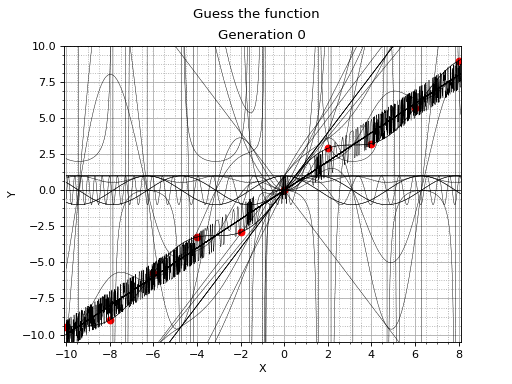
\includegraphics[width=0.2\linewidth]{images/foo-0.png}
	\caption{Symbolische Regression mit genetischer Programmierung}
	\label{fig::sym}
\end{figure}
\begin{figure}[h]
\centering
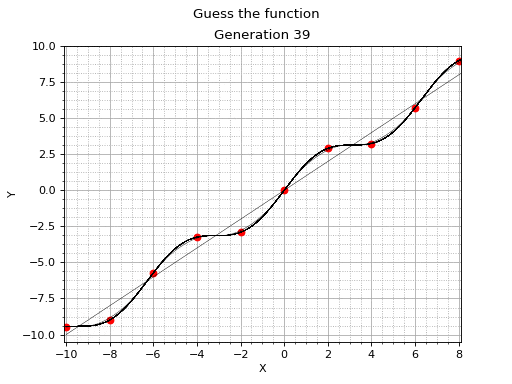
\includegraphics[width=0.2\linewidth]{images/foo-39.png}
\caption{Symbolische Regression mit genetischer Programmierung nach 39 Generationen}
\label{fig::gen}
\end{figure}
\section{Lösungsansatz}
Jeder mathematische Ausdruck kann in Form eines Syntaxbaums dargestellt werden. Ss gibt unendlich viele verschiedene Syntaxbäume, die semantisch äquivalenten Ausdrücken entsprechen. Zum Beispiel:
\begin{figure}[h]
	 \centering
	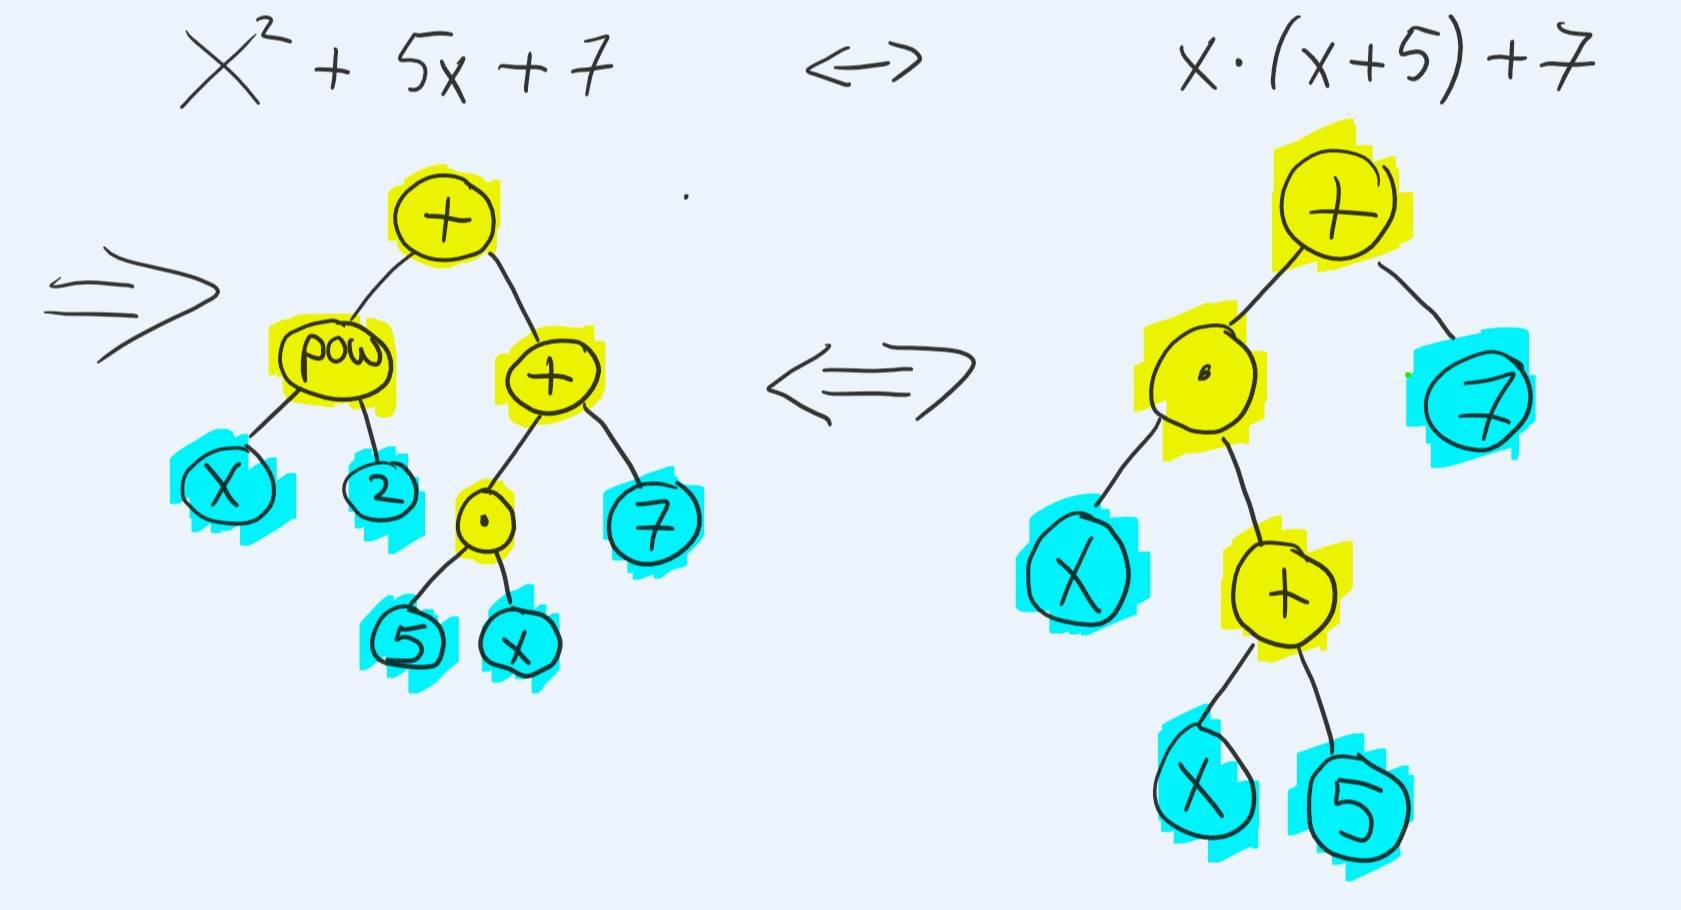
\includegraphics[width=0.4\linewidth]{matextree.jpg}
	\caption{Mathematischer Ausdruck als Syntaxbaum}
	\label{fig::matextree}
\end{figure}

In Bezug auf den genetischen Algorithmus:
\begin{enumerate}
	\item  kann jeder Syntaxbaum als "Chromosom" behandelt werden (eine Einheit, die "mutieren" und sich durch "Crossover" mit anderen "Chromosomen" verändern kann).
	\item Es ist notwendig, eine Fitnessfunktion zu definieren: die Funktion, die berechnet, wie gut jede Formel (die durch den Syntaxbaum kodiert wurde) - die vorhandenen Daten repräsentieren kann (z.B.: mit dem mittleren quadratischen Fehlerwert).
\end{enumerate}


\begin{figure}[h]
	\centering
	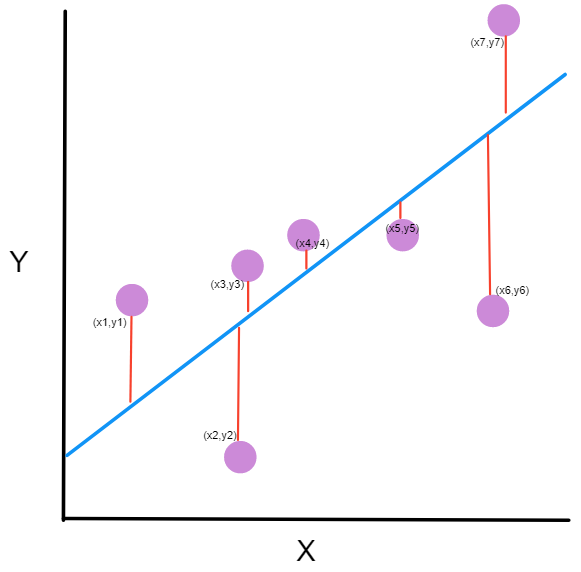
\includegraphics[width=0.4\linewidth]{mse.png}
	\caption{Mittlerer quadratischer Fehlerwert}
	\label{fig::mse}
\end{figure}
\newpage
\subsubsection{Crossover}
Beim "Crossover" wird der Syntaxbaum durch die Substitution seines Teilbaums durch einen Teilbaum eines anderen Syntaxbaums verändert.
\\
Das folgende Bild erklärt die Implementierung der "Crossover"-Operation über Syntaxbäume:


\begin{figure}[h]
	\centering
	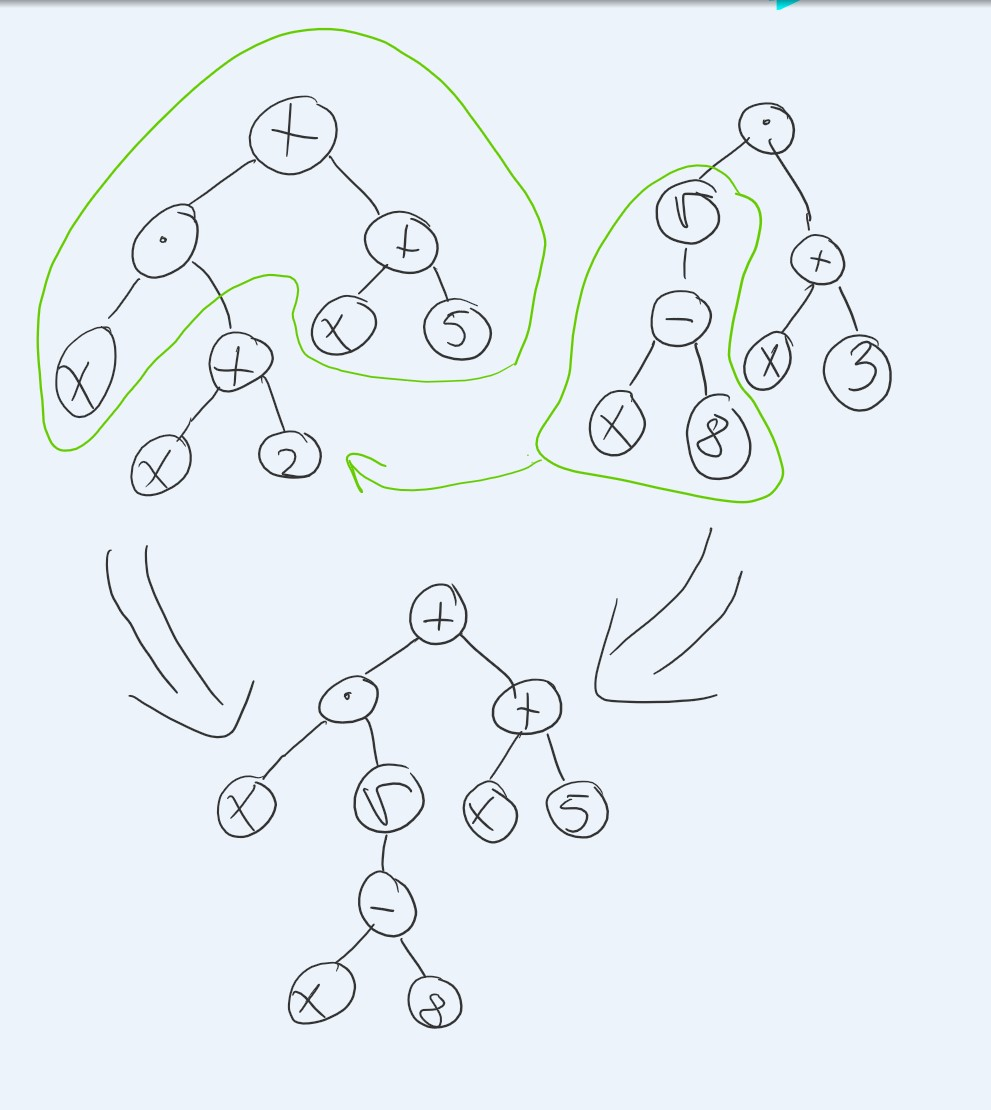
\includegraphics[width=0.25\linewidth]{crossover.jpg}
	\caption{Crossover Funktionsweise}
	\label{fig::cross}
\end{figure}

\subsubsection{Mutation}
Bei der Mutation wird es verschiedene Operationen geben:
\begin{itemize}
	\item Ersetzen eines Knotens des Syntaxbaums durch einen Knoten, der einer anderen Rechenoperation entspricht
	\item Ersetzen eines Teilbaums durch einen zufällig erzeugten Teilbaum
\item Entfernen eines Zwischenknotens aus dem Syntaxbaum
\item Erweitern des Baums von der Wurzel aus
\item Vertauschen von Teilbäumen bei nicht-kommutativen Oparationen

\end{itemize}
Beispielhaft habe ich mal das ersetzen eines Sub Baumes skizziert


\begin{figure}[h]
	\centering
	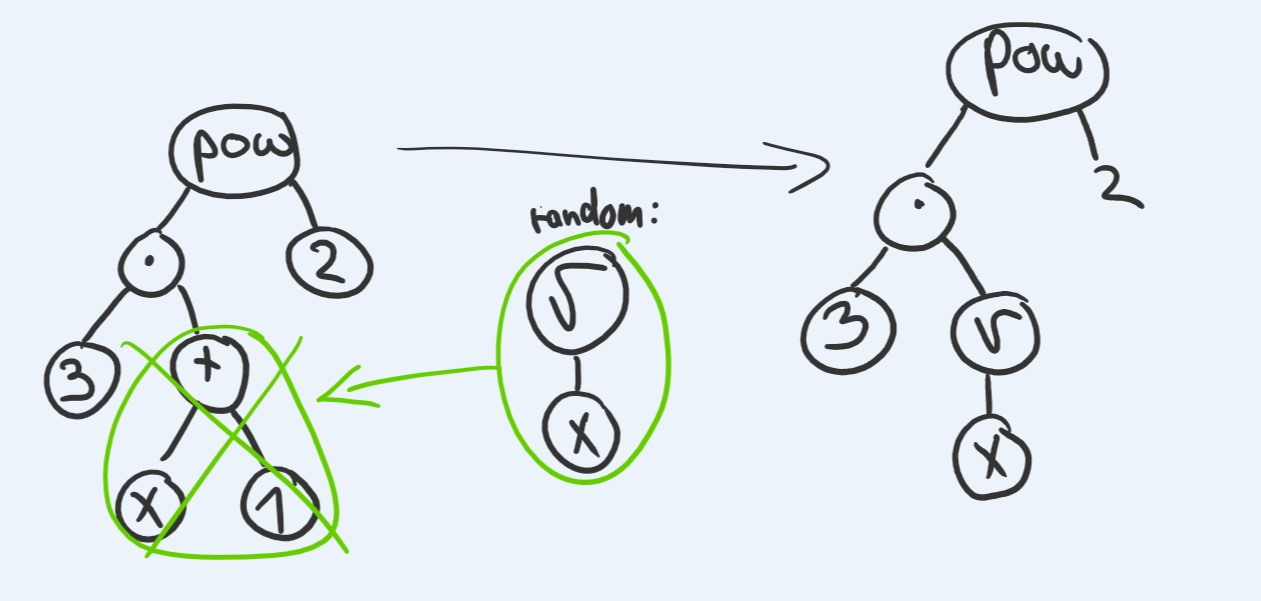
\includegraphics[width=0.4\linewidth]{mutationswap.jpg}
	\caption{Crossover Funktionsweise}
	\label{fig::mut}
\end{figure}

\subsection{Implementation}
Meine erste Wahl wäre Python gewesen, da ich in Python die Besten Kenntnisse besitze. 
Python  bietet eine Menge interessanter Bibliotheken für genetische Algorithmen und dezente Plotting-Funktionen. Einige der beliebtesten Bibliotheken sind Pyvolution, deap, pySTEP, PyRobot, DRP und mehr. Diese Bibliotheken sind in der Lage, eine interaktive Grafik-Demo-Anwendung bereitzustellen.
Ich habe aber auch die Idee es eventuell irgendwann als ReactJs Anwendung zur Verfügung zu stellen, da ich noch eine Domain besitze und es auch hosten könnte.
\section{Informationen zum Nachschlagen}
Symbolic regression via genetic programming, by D.A. Augusto; H.J.C. Barbosa : 
\url{
	https://ieeexplore-ieee-org.ezproxy.htwk-leipzig.de/stamp/stamp.jsp?tp=&arnumber=889734}


\section{Alternativer Vorschlag - Kantenerkennung mit evolutionären Algorithmen}


In dem Paper "Edge detection using evolutionary algorithms" by C.M. Ng; W.N. Leung; F. Chun wurde vorgestellt, wie man mithilfe evolutionärer Algorithmen Kanten erkennen kann. Eine grafische Oberfläche dazu zu bauen könnte in der Lehre eingesetzt werden und würde bestimmt Spaß machen.  
\url{https://ieeexplore.ieee.org/abstract/document/812522}

\begin{figure}[h]
	\centering
	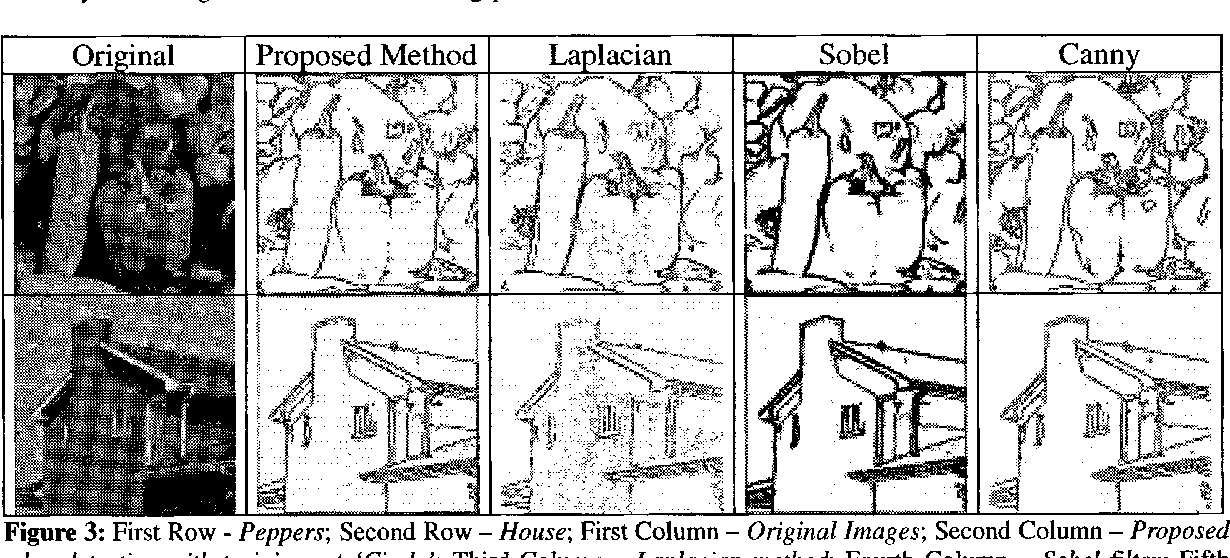
\includegraphics[width=0.4\linewidth]{geneticcanny.png}
	\caption{Kantenerkennung mit evolutionären Algorithmen}
	\label{fig::can}
\end{figure}

Sind diese Projektideen passend? Welche wäre Ihrer Erfahrung nach realistischer und besser geeignet als Projekt? Wenn keines der Beiden in Frage kommt, können sie mir eines zuweisen.
\end{document}